\chapter{Encoding axiomatic set theory}
\label{chap:sets}

The treatment of equational reasoning in the previous chapter introduced the ways in which Jape can hide parts of a proof and use substitution to achieve replacement of subformulae with rewrite rules. This chapter shows how the same techniques can be used to support the encoding of a version of naive axiomatic set theory, which uses rewriting to support equality-style reasoning in both forward and backward steps. The treatment was inspired by that of David Schmidt (``Natural Deduction Theorem Proving in Set Theory'', CSR-142-83, Edinburgh); like \chapref{ItL} this was an encoding to support a lecture course at QMW, commissioned by the lecturer.

\var{formula}
The encoding presents four distinct things to the user: an encoding of natural deduction, as a menu of commands; an menu of rewrite actions; a menu of set-theoretic inference rules; and a panel of axioms expressed as definitions $\<formula> \hat{=} \<formula>$, equipped with buttons which allow those definitions to be used as left-to-right or right-to-left rewrite rules. In addition there's a menu of conjectures equipped with buttons which allow the user to exploit proved theorems as rewrite rules.

In its time this was the most ambitious use of Japeish so far to produce a slick on-screen encoding with a lot of different --- but easy to use --- facilities. The encoding can hardly be described as `transparent'. The tactic programming is, indeed, at times rather subtle.

\section{The natural deduction encoding}

This is contained in the files \texttt{examples/Barwise\_n\_Etchemendy/BnE-Fprime.jt} and the files that it invokes; it is derived from the logic $F'$ in ``\emph{The Language of First-Order Logic}'' by Barwise and Etchemendy. It is very similar to the encoding described in \chapref{ItL} above, with the addition of rules for a bi-implication operator, a falsity constant, equality, and a unique-existence operator:\\

\begin{ruletab}{|l|l|l|} 
\hline
% ROW 1
$\infer[\reason{$<->-I$}]
       {\Gamma  |- A<->B}
       {\Gamma,A |- B\quad \Gamma,B |- A}$  
& 
$\infer[\reason{$<->-E(L)$}]
       {\Gamma  |- A}
       {\Gamma  |- B\quad \Gamma  |- A<->B}$ 
& 
$\infer[\reason{$<->-E(R)$}]
       {\Gamma  |- B}
       {\Gamma  |- A\quad \Gamma  |- A<->B}$ \\
\hline
% ROW 2
$\infer[\reason{$\bot -I$}]
       {\Gamma  |- \bot }
       {\Gamma  |- P\quad \Gamma  |- !P}$
&
$\infer[\reason{$\bot -E$}]
       {\Gamma  |- P}
       {\Gamma  |- \bot }$
& 
$\infer[\reason{$A=A$}]
       {\Gamma  |- A=A}
       {}$ \\
\hline
% ROW 3
\multicolumn{2}{|l|} {
$\infer[\reason{(\textsc{fresh} $c$, $c$ \textsc{notin} B) $|*\text{!} -E$}]
       {\Gamma  |-|*\text{!}x.A}
       {\Gamma  |- A[x\backslash B]\quad \Gamma,A\lbrack x\backslash c] |- B=c}$ } 
&
$\infer[\reason{$|*\text{!}-E$}]
       {\Gamma  |-|*x.A}
       {\Gamma  |-|*\text{!}x.A}$\\
\hline 
\end{ruletab}


plus a pair of rewrite rules for each of the bi-implication and equality operators:

\begin{ruletab}{|l|l|} 
\hline
% ROW 1
$\infer[\reason{$rewrite\,<->\,$}]
       {\Gamma  |- P[v\backslash A]}
       {\Gamma  |- A<->B\quad \Gamma  |- P\lbrack v\backslash B]}$ 
& 
$\infer[\reason{$rewrite\,<->\,$}]
       {\Gamma  |- P[v\backslash B]}
       {\Gamma  |- A<->B\quad \Gamma  |- P\lbrack v\backslash A]}$ \\
\hline
% ROW 2
$\infer[\reason{$rewrite\,=\,$}]
       {\Gamma |- P[v\backslash A]}
       {\Gamma  |- A=B\quad \Gamma  |- P[v\backslash B]}$  
&
$\infer[\reason{$rewrite\,=\,$}]
       {\Gamma |- P[v\backslash B]}
       {\Gamma  |- A=B\quad \Gamma  |- P[v\backslash A]}$ \\
\hline 
\end{ruletab}


These are encoded, completely straightforwardly, in the file \texttt{examples/Barwise\_n\_Etchemendy/BnE-Fprime\_rules.j}. The rules are inserted into the menu as
\begin{quote}\tt\small
MENU "System F´" IS\\
\tab ENTRY "→-I" \\
\tab ENTRY "↔-I"\\
\tab ENTRY "∧-I" \\
\tab ENTRY "∨-I(L)" IS FOB ForwardCut 0 "∨-I(L)"\\
\tab ENTRY "∨-I(R)" IS FOB ForwardCut 0 "∨-I(R)"\\
\tab ENTRY "¬-I"\\
\tab ENTRY "⊥-I"\\
\tab ENTRY "∀-I"\\
\tab ENTRY "∃-I" IS "∃-I tac"\\
\tab ENTRY "∃!-I" IS "∃!-I tac"

\tab SEPARATOR

\tab ENTRY "→-E"     IS "→-E tac" \\
\tab ENTRY "↔-E(L)"  IS FOB "↔-E(L) forward" 0 "↔-E(L)" \\
\tab ENTRY "↔-E(R)"  IS FOB "↔-E(R) forward" 0 "↔-E(R)" \\
\tab ENTRY "∧-E(L)"  IS FOB ForwardCut 0 "∧-E(L)"\\
\tab ENTRY "∧-E(R)"  IS FOB ForwardCut 0 "∧-E(R)"\\
\tab ENTRY "∨-E"     IS "∨-E tac"    \\
\tab ENTRY "¬-E"     IS FOB ForwardCut 0 "¬-E"   \\
\tab ENTRY "⊥-E"     IS FOB ForwardCut 0 "⊥-E"   \\
\tab ENTRY "∀-E"     IS "∀-E tac"    \\
\tab ENTRY "∃-E"     IS "∃-E tac"\\
\tab ENTRY "∃!-E(∃)" IS FOB ForwardCut 0 "∃!-E(∃)"\\
\tab ENTRY "∃!-E(∀∀)"    IS FOB ForwardCut 0 "∃!-E(∀∀)"

\tab SEPARATOR

\tab ENTRY "A=A"\\
\tab ENTRY hyp       IS hyp
END
\end{quote}

Here \texttt{fob} is essentially the tactic \texttt{ForwardOrBackward} of \chapref{ItL}, \texttt{ForwardCut} and \texttt{ForwardUncut} are also as described there, and the entries for bi-implication use the tactics
\begin{japeish}
TACTIC "↔-E(L) forward"(Z) IS "↔-E forward" "↔-E(L)" \\
TACTIC "↔-E(R) forward"(Z) IS "↔-E forward" "↔-E(R)"\\
\\
TACTIC "↔-E forward"(rule) IS\\
\tab WHEN (LETHYP (\_A↔\_B) (ForwardCut2 rule))\\
\tab \tab (LETHYP \_A (ForwardCut rule))\\
\tab \tab (JAPE(fail(what's this in rule forward?)))
\end{japeish}

Using the rewrite rules is, as we have seen in \chapref{funcprog}, a little more complicated. The Substitution menu is
\begin{japeish}
MENU "Substitution" \\
\tab ENTRY "A↔\dots"     IS ForwardSubst "rewrite ↔ «" "rewrite ↔ »" (↔) \\
\tab ENTRY "\dots↔B"     IS ForwardSubst "rewrite ↔ »" "rewrite ↔ «" (↔) \\
\tab ENTRY "A=\dots"     IS ForwardSubst "rewrite = «" "rewrite = »" (=) \\
\tab ENTRY "\dots=B"     IS ForwardSubst "rewrite = »" "rewrite = «" (=) \\
END
\end{japeish}

The ForwardSubst tactic extends the techniques of \chapref{funcprog} to allow rewriting in forward as well as backward reasoning style. We require that the user must subformula-select some subformula and also may select a hypothesis which is to be used as $A=B$ or $A<->B$ in the rule. The tactic is rather subtle:\footnote{You might wonder whether the complexity of this tactic programming doesn't undermine the claim that Jape is simple and easy to program. Well, yes it does. But I now realise that while encoding the rules of a logic in Jape and arranging them in menus is straightforward and transparent, the work required to hide parts of proofs or to achieve concise effects by hiding gestures is programming, and programming is always potentially intricate.} it's given a left-to-right rewrite rule \textit{ruleLR}, a right-to-left rewrite rule \textit{ruleRL}, and a pattern \textit{pat} which it uses in error alerts. Note how the menu entries alternate the use of the rewrite rules to get the correct rewriting effect when working either forward or backwards.

\begin{japeish}
TACTIC ForwardSubst (ruleLR, ruleRL,pat) IS\\
\tab WHEN \\
\tab \tab (LETHYPSUBSTSEL \_P \\
\tab \tab \tab cut\\
\tab \tab \tab ruleRL \\
\tab \tab \tab (WHEN \\
\tab \tab \tab \tab (LETHYP \_Q \\
\tab \tab \tab \tab \tab (ALT (WITHHYPSEL hyp) \\
\tab \tab \tab \tab \tab \tab (FAIL (the hypothesis you formula-selected wasn't a pat formula))))\\
\tab \tab \tab \tab (JAPE (SUBGOAL 1))) \\
\tab \tab \tab (WITHSUBSTSEL hyp))\\
\tab \tab (LETCONCSUBSTSEL \_P\\
\tab \tab \tab (WITHSUBSTSEL ruleLR)\\
\tab \tab \tab (WHEN \\
\tab \tab \tab \tab (LETHYP\_Q \\
\tab \tab \tab \tab \tab (ALT (WITHHYPSEL hyp) \\
\tab \tab \tab \tab \tab \tab (FAIL(the hypothesis you formula-selected wasn't a pat formula))))\\
\tab \tab \tab \tab SKIP))\\
\tab \tab (JAPE (fail(please text-select one or more instances of a sub-formula to replace)))
\end{japeish}

\textsc{lethypsubstsel} \textit{pattern tactic...} succeeds when the user's subformula-selections describe a substitution in a hypothesis (left-hand side) formula; \textsc{letconcsubstsel} succeeds when they describe a substitution in a conclusion (right-hand side). Working backwards with letconcsubstsel the tactic is fairly straightforward: it applies ruleLR (one of the argument rewrite rules) on the substution formula that the user has defined, and then, if the user has selected a hypothesis, tries to unify it with the conclusion of the first antecedent of the rewrite. Working forwards it makes a cut, applies ruleRL (the other rewrite rule, which will do its work in the opposite direction to ruleLR) and then either applies the user's selected hypothesis (alt...) or skips the first antecedent (jape(subgoal 1)) and then does \textsc{withsubstsel} hyp, which uses the user's original subformula-selection to construct a substitution in the current problem sequent, and also does an automatic \textsc{withhypsel} on it, so that the hyp is bound to make use of that hypothesis\.footnote{It seems reasonable that withsubstsel should include an automatic withhyp/withconcsel, because if the newly-constructed hypothesis isn't to be used, why was it constructed?} The automatic \textsc{withhypsel} enables us, as in this example, to distinguish between two selected hypotheses: the one selected for application as an equality, and the one subformula-selected for rewriting.\footnote{The encoding uses the out-of-date terminology `text selection', because it was written before subformula selection was implemented, when all you could do was select character sequences.}

\section{Syntax of set operations}

Apart from the various operators, which have been encoded in the obvious way, the only important syntactic feature of this encoding is the treatment of \emph{set abstractions}. Jape's parser-generator isn't very sophisticated, so I had to make some drastic simplifications.

The form of a set abstraction, in this encoding, is $\{ \mathit{variable} | \mathit{formula} \}$, and the occurrence of the variable to the left of the bar is a binding occurrence; I also allow $\{ \texttt{<}\mathit{variable},\mathit{variable}\texttt{>} | \mathit{formula} \}$. I include, therefore, in \texttt{set\_syntax.j}
\begin{japeish}
CLASS VARIABLE u v w \\
CONSTANT Ø ⊥ U EQ \\
\\
PREFIX  1000            Pow \\
PREFIX  800             ∪∪ ∩∩ \\
POSTFIX 800             ⁻¹ \\
INFIX           700L            ∪ ∩ - \\
INFIX           720L            • \\
INFIX           740L            × \\
INFIX           600L            ⊆ \\
INFIX           500L            ∈ ∉ \\
\\
OUTFIX < > \\
OUTFIX { } \\
OUTFIX { | } \\
 \\
BIND y SCOPE P IN { y | P } \\
BIND x y SCOPE P IN { <x,y> | P }
\end{japeish}
The priority numbers chosen are higher than the priority of any operator in \texttt{BnE-Fprime\_syntax.j}, and otherwise have no particular significance. 

Given the \textsc{outfix} and \textsc{bind} directives above, together with the standard interpretation of comma as a zero-priority associative operator, the encoding recognises the following formula-shapes:
\begin{description}
\item[$\{\,\}$] the empty set;
\item[$\{ \mathit{formula} \}$] a singleton set;
\item[$\{ \mathit{formula},\dots,\mathit{formula} \}$] a literal description of a set;
\item[$\{ \mathit{variable} \mid \mathit{formula} \}$] a set abstraction;
\item[$\{ <\!\mathit{variable}, \mathit{variable}\!> \mid \mathit{formula} \}$] an abstraction of a set of pairs.
\end{description}
Allowing set brackets with or without the vertical bar is a trick of which I was once ashamed.

\section{The axiomatic presentation of naive set theory}

We first observe, just to get it out of the way, that this encoding of set theory does not attempt to avoid Russell's paradox (see \texttt{sets\_russell.j}). Schmidt's treatment was based on G\"{o}del-Bernays set theory and had a judgement ``Set $A$'', which I didn't duplicate, principally because my client didn't want me to.

The axioms of comprehension and extension in this naive treatment are
\begin{description}
\item[comprehension] $@*P.|*A.x\in A<->P(x)$;
\item[extension] $@*A,B.\,A=B<->(@*x.x\in A<->x\in B)$
\end{description}
Comprehension isn't first order, but it's encoded in rules which are implicitly-quantified schemata so that's ok. I couldn't find a way to incorporate comprehension as a single rule, because of the existence operator, and so I followed Schmidt and incorporated it as two rules for each of the set-abstraction forms:
\begin{ruletab}{|l|l|} 
\hline
% ROW 1
$\infer
       {\Gamma  |- A\in \{ y \mid P( y) \} }
       {\Gamma  |- P(A) }$ 
& 
$\infer
       {\Gamma |- P(A) }
       {\Gamma  |- A\in \{ y \mid P( y) \} } $
\\
\hline 
$\infer
       {\Gamma  |- <\! A,B\!> \in \{ <\!y,z\!>  \mid P(y,z) \} }
       {\Gamma  |- P(A,B) }$ 
& 
$\infer
       {\Gamma  |- P(A,B) }
       {\Gamma  |- <\! A,B\!> \in \{ <\! y,z\!>  \mid P( y,z) \} }$
\\
\hline 
\end{ruletab}

The rules are encoded as a couple of \textsc{alt}s
\begin{japeish}
RULES "abstraction-I"(A, OBJECT y,OBJECT z) ARE  \\
\tab \tab FROM P(A) INFER A∈{ y | P(y) } \\
\tab AND FROM P(A,B) INFER <A,B>∈{ <y,z> | P(y,z) } \\
END \\
RULES "abstraction-E"(A, OBJECT y, OBJECT z) ARE \\
\tab \tab FROM A∈{ y | P(y) } INFER P(A)  \\
\tab AND FROM <A,B>∈{ <y,z> | P(y,z) } INFER P(A,B) \\
END
\end{japeish}
(\texttt{BnE-Fprime.jt} sets \texttt{interpretpredicates} true, so $P(A)$ is really shorthand for a substitution).
and are incorporated into the SetOps menu in the usual way
\begin{japeish}
ENTRY "abstraction-I" IS FSSOB ForwardCutwithSubstSel "abstraction-I"\\
ENTRY "abstraction-E" IS FOBSS ForwardCut "abstraction-E"
\end{japeish}

The \textsc{fobss} and \textsc{fssob} tactics are each a variation of the \textsc{fob} tactic, requiring that the user makes a text selection when reasoning backward (\textsc{fobss}) or forward (\textsc{fssob}):
\begin{japeish}
TACTIC FOBSS (Forward, Rule) IS \\
\tab WHEN\tab (LETHYP \_P\\
\tab \tab \tab (ALT\tab (Forward Rule)\\
\tab \tab \tab \tab (WHEN\tab (LETARGSEL \_Q \\
\tab \tab \tab \tab \tab \tab (JAPE(failgivingreason(Rule is not applicable to assumption ' \_P ' \\
\tab \tab \tab \tab \tab \tab \tab \tab \tab \tab with argument ' \_Q '))))\\
\tab \tab \tab \tab \tab (JAPE(failgivingreason(Rule is not applicable to assumption ' \_P ')))))) \\
\tab \tab (LETCONCSUBSTSEL \_P \\
\tab \tab \tab (ALT\tab (WITHSUBSTSEL (WITHHYPSELRule))\\
\tab \tab \tab \tab (LETGOAL \_Q\\
\tab \tab \tab \tab \tab (JAPE(failgivingreason(Rule is not applicable to conclusion ' \_Q '\\
\tab \tab \tab \tab \tab \tab \tab \tab \tab \tab with substitution ' \_P '))))))\\
\tab \tab (ALT\tab (WITHSELECTIONS Rule)\\
\tab \tab \tab (JAPE(failgivingreason(Rule is not applicable to that conclusion)))) \\
\\
TACTIC FSSOB (Forward, Rule) IS \\
\tab WHEN\tab (LETHYPSUBSTSEL \_P (Forward Rule)) \\
\tab \tab (ALT\tab (WITHSELECTIONS Rule)\\
\tab \tab \tab (WHEN\tab (LETARGSEL \_P\\
\tab \tab \tab \tab \tab (JAPE(failgivingreason(Rule is not applicable with argument ' \_P '))))\\
\tab \tab \tab \tab (JAPE(failgivingreason(Rule is not applicable))))) \\
\\
TACTIC ForwardCutwithSubstSel(Rule) IS\\
\tab SEQ\tab cut \\
\tab \tab (WHEN\tab (LETSUBSTSEL \_A Rule (WITHSUBSTSEL hyp))\\
\tab \tab \tab \tab (JAPE (fail(please text-select one or more instances of a sub-formula))))
\end{japeish}

I incorporate extension as an axiomatic definition. I don't include the outer quantification, as rules are implicitly-quantified schemata. It's encoded in the Definitions panel (see below) as
\begin{japeish}
RULE (OBJECT y) IS A=B ≜ (∀y.y∈A↔y∈B)
\end{japeish}
When we use this rule we will normally do so with a rewrite: replace some subformula which matches one side or other of the definition, closing the first antecedent of the rewrite with an instance of the definition. But we don't want to see the particular instance of the axiom as part of the proof: just as in the functional programming example, it is best referred to in the justification of the rewrite step, and otherwise hidden from view.

I include the rule as part of a Definitions panel, and have two buttons on the panel which allow left-to-right and right-to-left rewriting. As with the Substitution menu, switching the rewrite rules around in the tactics associated with each button allows forward or backward rewriting, The panel definition is in \texttt{BnE-Fprime\_menus.j}:
\begin{japeish}
TACTICPANEL "Definitions" IS \\
\tab RULE INFER A≠B ≜ ¬(A=B) \\
\tab  \\
\tab BUTTON "A≜…" IS apply ForwardSubstHiding "rewrite ≜ «" "rewrite ≜ »"  COMMAND \\
\tab BUTTON "…≜B" IS apply ForwardSubstHiding "rewrite ≜ »" "rewrite ≜ «"  COMMAND \\
END
\end{japeish}

The tactic ForwardSubstHiding allows the user to rewrite
\begin{itemize}
\item either a hypothesis or a conclusion;
\item after subformula-selecting a number of instances of a subformula, just those instances;
\item without subformula-selecting, the whole hypothesis or conclusion.
\end{itemize}

In fact it is only forward rewriting without text selection that is more subtle than what we have already seen.
\begin{japeish}
TACTIC ForwardSubstHiding (ruleLR, ruleRL, thm) IS \\
\tab WHEN     \\
\tab \tab (LETHYPSUBSTSEL \_P  cut (LAYOUT thm (1) ruleRL thm (WITHSUBSTSEL hyp))) \\
\tab \tab (LETCONCSUBSTSEL \_P (LAYOUT thm (1) (WITHSUBSTSEL ruleLR) thm)) \\
\tab \tab /* the "second argument" of the rewrite rules has to be B */ \\
\tab \tab (LETHYP \_P cut (LAYOUT thm (1) (ruleRL[B{\textbackslash}\_P]) thm (WITHHYPSEL hyp))) \\
\tab \tab (LETGOAL \_P (LAYOUT thm (1) (ruleLR \_P) thm)) \\
\end{japeish}
The first alternative is activated when the user has subformula-selected in a hypothesis: it cuts, uses one of the rewrite rules, closes the first antecedent with the theorem, and the second using the subformula-selection that the user made. The second alternative is activated when there is a subformula-selection in a conclusion: it uses the other rewrite rule followed by the theorem. The last alternative is activated when there is no recognisable subformula-selection and no hypothesis selection: it activates the same rewrite rule as the second alternative, but gives it the whole conclusion formula instead of the user's text selection: that is a particularly easy `abstraction' for the substitution-unifier to resolve, and the effect is to unify the whole consequent with the left- or the right-hand side of the theorem, depending on the particular rewrite rule that is used.

The third alternative is the tricky one. It calls the same rewrite rule as the first alternative, but gives it the selected hypothesis as argument $B$. The rule has to be something like
\begin{japeish}
RULE "rewrite ≜ «" (A) IS FROM A≜B AND P(B) INFER P(A)
\end{japeish}
But the instantiation says nothing about $A$, so that rule will necessarily succeed by deferred unification of $\_P'[v{\backslash}\_A]$ with the conclusion. Then it closes the first antecedent of the rewrite with the theorem which has to match $A≜B$ and therefore tells it what $\_A$ is: but we still don't know $\_P'$. After the theorem is applied, the second antecedent of the rewrite step will be $\_P'[v{\backslash}B]$: using hyp we unify that with $\_P$, which is $B$, and the effect is just like the fourth alternative (and surely I ought to have written the fourth alternative as
\begin{japeish}
(LETGOAL \_P (LAYOUT thm (1) (ruleLR[A{\textbackslash}\_P]) thm))
\end{japeish}
--- but it was composed in the days before you could write that kind of rule application, and I didn't think to update it).

Each of the entries in the Definitions panel is intended to be used as a two-way rewrite rule, using the buttons as described above. Note that I've had to include definitions of negated operators like ≠ and ∉ in terms of negated formulae.\footnote{I always wanted to do this sort of thing by `definitional equality', where you write $A!=B$ and Jape interprets it as $¬(A=B$) but still displays what you wrote. I never managed it.}. The set additions are defined in \texttt{set\_menus.j}; the \textsc{object} qualifiers are for convenience, so that you don't get too many unknowns in your proof:\footnote{Nowadays Jape can use alpha-conversion of binding forms when unifying, so the fresh variables don't really get in the way.}
\begin{japeish}
TACTICPANEL "Definitions" IS \\
\tab RULE IS A∉B ≜ ¬(A∈B) \\
\tab RULE IS Ø ≜ \{\} \\
\tab RULE (OBJECT x) IS EQ ≜ \{x|x=x\} \\
\tab RULE (OBJECT x) IS \{A\} ≜ \{x|x=A\} \\
\tab RULE (OBJECT x) IS \{A,B\} ≜ \{x|x=A∨x=B\} \\
\tab RULE (OBJECT x) IS \{A,B,C\} ≜ \{x|x=A∨x=B∨x=C\} \\
\tab RULE (OBJECT x) IS \{A,B,C,D\} ≜ \{x|x=A∨x=B∨x=C∨x=D\} \\
\tab RULE (OBJECT y) IS A⊆B ≜ (∀y.y∈A→y∈B) \\
\tab RULE (OBJECT y) IS A=B ≜ (∀y.y∈A↔y∈B) \\
\tab RULE (OBJECT y) IS A∪B ≜ \{ y | y∈A∨y∈B \} \\
\tab RULE (OBJECT y) IS A∩B ≜ \{ y | y∈A∧y∈B \} \\
\tab RULE (OBJECT y) IS A-B ≜ \{ y | y∈A∧y∉B \} \\
\tab RULE (OBJECT y) IS A⁻¹ ≜ \{y | y∉A\} \\
\tab RULE (OBJECT x, OBJECT y) IS ∪∪(C) ≜ \{ x | ∃y. x∈y∧y∈C \} \\
\tab RULE (OBJECT x, OBJECT y) IS ∩∩(C) ≜ \{ x | ∀y. y∈C→x∈y \} \\
\tab RULE (OBJECT x) IS Pow(A) ≜ \{ x | x⊆A \} \\
\tab RULE (OBJECT x, OBJECT y) IS A×B ≜ \{ <x,y>  | x∈A∧y∈B \} \\
\tab RULE (OBJECT x, OBJECT y, OBJECT z) IS A•B ≜ \{ <x,z> | ∃y.<x,y>∈A∧<y,z>∈B \} \\
END
\end{japeish}

\begin{figure}[htbp]
\centering
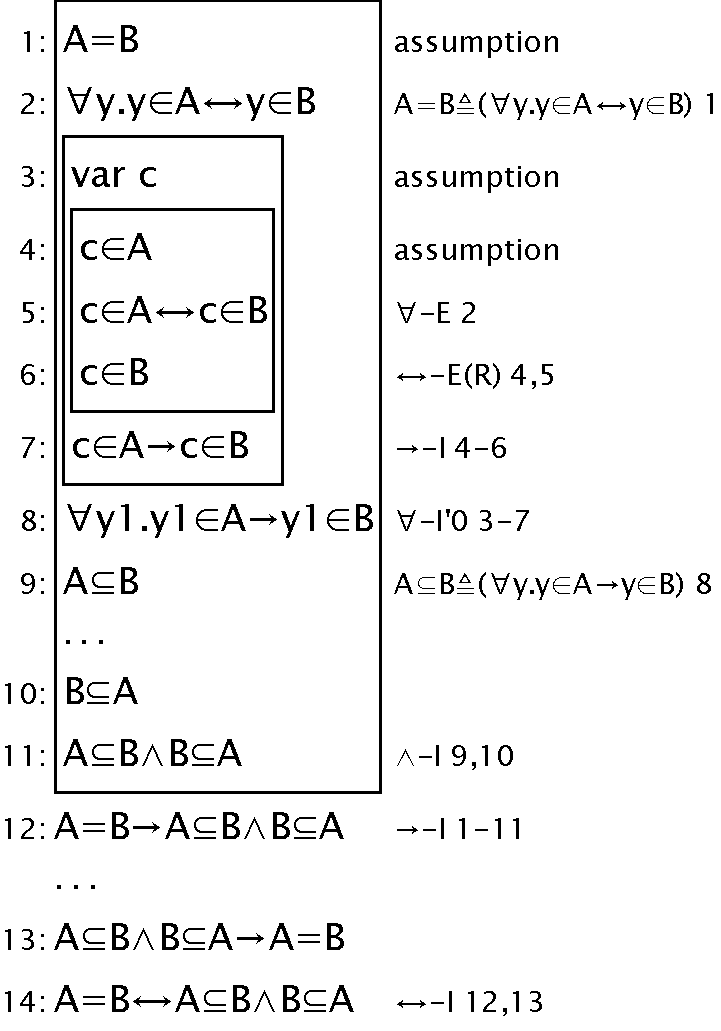
\includegraphics[scale=0.5]{pics/sets/axiomaticwasteful}
\caption{Beginning of a proof using logical rules and axiomatic definitions}
\label{fig:sets:axiomaticwasteful}
\end{figure}

\section{The non-axiomatic rules}

A proof using the axioms will typically introduce and then eliminate logical connectives. \Figref{sets:axiomaticwasteful} shows the beginning of such a proof. It is clear that there will be lots of repetitive applications of ∀-E, ∀-I, →-E, →-I, and similar logical rules during this proof. It is clear that there could be introduction and elimination rules for each of the set operators. These are the ones relevant to the proof above:
\begin{ruletab}{|l|l|l|} 
\hline
% ROW 1
$\infer[\reason{$(\operatorname{FRESH}\;c)\;\subseteq -I$}]
       {\Gamma  |- A\subseteq B}
       {\Gamma,c\in A |- c\in B}$ 
& 
$\infer[\reason{$\subseteq -E$}]
       {\Gamma |- C\subseteq B}
       {\Gamma  |- C\in A\quad \Gamma  |- A\subseteq B}$
& \\
\hline
% ROW 2
$\infer[\reason{$=-I$}]
       {\Gamma |- A=B}
       {\Gamma  |- A\subseteq B\quad \Gamma  |- B\subseteq A}$
& 
$\infer[\reason{$=-E(L)$}]
       {\Gamma  |- A\subseteq B}
       {\Gamma  |- A=B}$
& 
$\infer[\reason{$=-E(R)$}]
       {\Gamma  |- B\subseteq A}
       {\Gamma  |- A=B}$ \\
\hline 
\end{ruletab}
\Figref{sets:derivedeconomical} shows the proof completed using these rules, rather than the axiomatic definitions. Somewhat simpler! The rules are encoded in the obvious way in \texttt{set\_menus.j}. They are described as \textsc{derived rule}, because they can be proved from the axioms, and in \figref{sets:derivedeconomical} as conjectured rules, because no proof of them had been provided when that proof was made.

\begin{figure}[htbp]
\centering
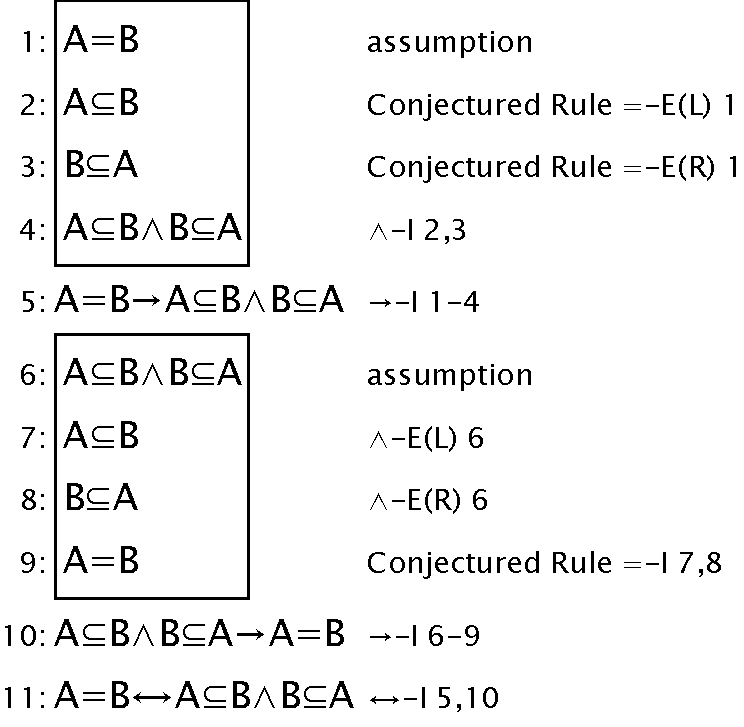
\includegraphics[scale=0.5]{pics/sets/derivedeconomical}
\caption{A proof using derived rules}
\label{fig:sets:derivedeconomical}
\end{figure}


 